% Copyright 2011, Piotr Jakubowski

\nocite{rest}

\chapter{Design and implementation}
  The aim of this chapter is to provide description of how the plugin codebase,
  show how it has been designed and what decisions has been made. In addition it aims to indicate
  interesting examples of usage of Ruby and Ruby on Rails API.
  
  \section{Overview}
    The plugin has been developed as Rails Engine (details will be covered in next chapter). This
    means that it is a Rails application that can be embedded into another one. The fact, that 
    the plugin is a Rails application provides the ability of using whole power of Ruby on Rails.
    So, it is possible to use the MVC pattern, set up routing for the application and so on.
    
    In order to get the plugin running following parts had to be developed:
    \begin{itemize}
      \item Setting the application as \texttt{Rails Engine} as said before.
      \item Handling the \texttt{Models} - finding all models in the application as well as
        getting the model class from string representation
      \item Getting the list of \texttt{Fields} in the model along with their type and any
        necessary attributes that would be necessary for generating the form for given model.
        This includes not only fields such as text or integer fields, but also handling associations
        between models which is the most challenging task.
      \item Elaborate a convenient way of defining \texttt{Configuration} for the plugin that would be both flexible
        and easy to use at the same time.
      \item Develop the web part of the plugin - setting up the \texttt{Routing, Controllers and Html Templates} that 
        would allow users to smoothly use the application.
    \end{itemize}
    
    The plugin has been developed along and tested with a simple application that would act like a simple blogging
    system. Appropriate features such as particular types of model associations has been added to the test application
    when needed in order to see whether the plugin handles it in correct way. As test application is not integral 
    part of the plugin it would not be described in details. In short, the models that would appear in the test application are
    following:
      \begin{description}
        \item[Posts] used as main model to test all associations on. It has standard fields such as string field for title,
          text field(long string) for body, date field for published at date.
        \item[Categories] can be attached to Post in association one-to-many. Used to test belongs\_to association in Post.
        \item[Comments] attached to Post in many-to-one association. Used to test has\_many association.
        \item[Attachment] attached to Post in one-to-one association. Used to test has\_one association.
      \end{description}
      
    Association testing has been shown from the Post model perspective, but the plugin would handle the associations
    from both ends as it needs to be universal and be working for every application.
    
  \section{Rails Engine}
    In order to create a web application that would be mountable into other Rails applications it has to be
    declared as an Engine. It can be obtained by defining an Engine class in the gem module:
    
    \lstinputlisting{code/chapter05/engine01.rb}
    
    This few lines of code makes the gem a Rails Engine. This means that it will load the code located in \texttt{app/} and 
    \texttt{config/} directories. This is acomplished by the single fact of creating a class that inherits from \texttt{Rails::Engine}
    as the internals of that class set up the load path for those directories. In fact, from version 3 of Rails every
    \texttt{Rails::Application} is \texttt{Rails::Engine}.
    
    Moreover, \texttt{Rails::Engine} or in fact its superclass \texttt{Rails::Railtie} enables developer to hook in into Rails
    initialization process by adding initializing routines to the list. This would become useful soon when the plugin would 
    need to do some actions after all Rails initialization has been done (will be covered in Fields chapter).
  \section{Models}
    A \texttt{Model} class is a central point of the administer plugin. It is responsible for handling models, getting the list of available models and so on.
    
    \subsection{Getting list of all models}
      First thing that needed to be done in respect of models was to find all models in the application. There are few possibilities of 
      obtaining the list of classes in current application. The first that has been tested was getting all subclasses of \texttt{ActiveRecord::Base}, which
      is a standard superclass for models in \texttt{ActiveRecord}:
      
      \lstinputlisting{code/chapter05/models01.rb}
    
      This works fine, but there is one thing that is not necessarily proper - hardcoding. It hardcodes the use of \texttt{ActiveRecord}. And, as the plugin
      should be as universal as possible, it is not a good idea to narrow the possibility of extending into other ORMs this early in implementation. Moreover,
      not all ORMs use a superclass as creating models. Some of them like \texttt{DataMapper}\footnote{http://datamapper.org/} or \texttt{Mongoid}\footnote{http://mongoid.org/}
      use a mechanism of including a module in a class so instead of:
    
      \lstinputlisting{code/chapter05/models02.rb}
  
      it becomes: 
    
      \lstinputlisting{code/chapter05/models03.rb}
      
      So there is a need for some other solution. Fortunately, Rails has a predefined structure of directories and it is known where the models (usually) are kept - 
      in \texttt{app/models} directory. Therefore, such an implementation has been derived:
      
      \lstinputlisting{code/chapter05/models04.rb}
      
      where \texttt{Model.for} is a method that returns a class with a name represented by given string. What this implementation does is - it looks for all \texttt{.rb}
      files in models directory and figures out models by looking at their names. This solution seems better as we no longer hardcode ActiveRecord. Howevwer,
      one more assumption here is done - usage of \texttt{app/models} as a directory for models. Since it is configurable in Rails it would be nice to handle
      the situations when the developer defined the models' directory to be something else. Fortunately, it is possible to get the configuration out of Rails.
      It can be obtained like that:
      
      \lstinputlisting{code/chapter05/models05.rb}
      
      Above implementation takes into account all directories defined in Rails as containers of models files by using \texttt{Rails.application.paths.app.models.paths.each}
    \subsection{Getting the class from string}
      As all parameters of HTTP request are in fact \texttt{Strings} there has to be a routine for changing a \texttt{String} into a \texttt{Class}. It is needed, because
      the user would in HTTP request define which resource he wants to access. One way would be to keep a hash where keys would be names of classes in string form and 
      values would be classes itself. But, since Ruby is a dynamic language with comprehensive reflection API that has been enriched with few methods by Rails it is possible
      to get it much smarter and have the implementation like this:
      
      \lstinputlisting{code/chapter05/models06.rb}
      
      It takes a string, camelizes it - which means \texttt{"my\_model"} would become \texttt{"MyModel"} and then calls \texttt{constantize} on that string. This method 
      (as described in 3.4.2) takes a string and returns a constant with that name.
      
      Then, in order to make the API flexible there is method \texttt{Model.for} defined that returns a \texttt{Model} instance for particular class

      \lstinputlisting{code/chapter05/models07.rb}
      
      Therefore it can be called either \texttt{Model.for("my\_model")} or \texttt{Model.for("MyModel")} or even \texttt{Model.for(MyModel)} if needed depending on a context.
      
  \section{Fields}
    Proper handling of fields of the model is probably the most tricky part of the application. If it was only
    for the fields in the database then it would not be that complex, but as the plugin is supposed to handle associations
    between models as well - that introduces the challenge.
    
    \subsection{Representation of fields in the system}
      At first there was an idea of passing around the list of fields for given model as the list of hashes.
      The hash for field would keep all information important for given type, so the most basic would keep:
        \begin{itemize}
          \item Name
          \item Type
        \end{itemize}
      and if needed it could keep other info, for example:
       \begin{itemize}
         \item Foreign Key
         \item Association Class
         \item Parent
        \end{itemize}
      
      The example of list of fields could look like:
      \lstinputlisting{code/chapter05/fields01.rb}
      
      However, such approach is not very flexible. If new type of field needs to be added the code for handling it
      should be changed in every place, where that list of hashes is accessed. Moreover, handling such list of hashes
      needs a lot of messy code itself, with a lot of conditions.
      
      Therefore, there emerged the need for some more comprehensive representation of the fields. More object oriented
      approach has been introduced. Every type of field would be represented by the class that would extend the most basic
      \texttt{Administer::Fields::Base}, which would provide the most fundamental constructor and set of methods. The
      hierarchy is presented in figure \ref{fields01} (page \pageref{fields01})
         
      \begin{figure}[hbt!]
    		\begin{center}
    			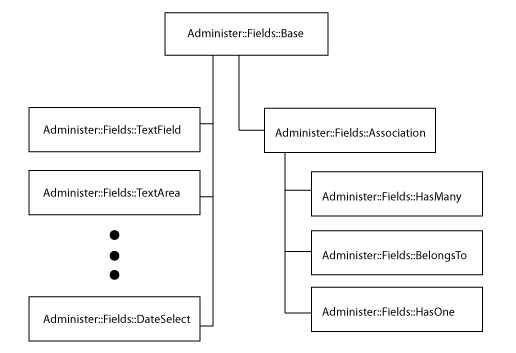
\includegraphics[width=0.8\linewidth]{images/chapter05/fields01.png}
    			\caption{Diagram of structure of classes representing fields}
    			\label{fields01}
    		\end{center}
    	\end{figure}
    
    \subsection{Mapping of actual fields into their representation}
      As there is already the structure that will represent the fields in the system, the only problem was to 
      map the actual fields and associations into what they should be. This process consists of two parts:
        \begin{itemize}
          \item Getting the list of fields and associations from the model
          \item Mapping to appropriate classes
        \end{itemize}

      \subsubsection{Getting the list of fields and associations from the model}
        ActiveRecord reflection API enables developer to get the list of all database fields for given
        model by using \texttt{columns} method. This returns the list of \texttt{ActiveRecord::ConnectionAdapters::Column}
        subclasess (depending on database adapter it would be \texttt{SQLiteColumn}, \texttt{PostgreSQLColumn} and so on).
        The \texttt{ActiveRecord::ConnectionAdapters::Column} class contains all kind of data for the column, but the most
        important from the perspective of the plugin is \texttt{name} and \texttt{type}. 
        
        The list contains all columns, which means that the foreign keys for \texttt{belongs\_to} associations
        are there as well. They would have to be substituted by the associations themselves.
        
        Moreover, in order to get the associations the \texttt{reflect\_on\_all\_associations} method can be used which 
        returns the list of all association reflections objects. They are represented by 
        \texttt{ActiveRecord::Reflection::AssociationReflection}, which contains information on the type of
        association, class of associated objects etc.
        
        After combining those lists together and replacing \texttt{belongs\_to} foreign keys columns with association
        representations the list is ready to be transformed into our representation of fields.

      \subsubsection{Mapping fields to appropriate representation classes}
        Next step is to map obtained objects into objects that would be useful for the purpose of rendering 
        form or displaying the list of records. For this purpose the \texttt{FieldBuilder} class has been introuced.
        Its responsibility is to keep rules for such mapping and perform the transition for given set of 
        fields. 
        
        Again, flexibility has been an issue here. In order to not hardcode the rules in the class, the interface for
        registering rules has been developed. The \texttt{FieldBuilder} class introduces \texttt{register\_class}
        method which takes two parameters - the class and the block that describes a mapping rule for given class.
        
        For instance, the definition of (shortened) rule for \texttt{Column} from \texttt{ActiveRecord} may be the
        following.
        
        \lstinputlisting{code/chapter05/fields02.rb}
    
        Those rules are kept in a special type of hash (from gem called 
        SuperclassHash\footnote{https://github.com/piotrj/superclass\_hash}, which has been developed 
        for the purpose of that plugin as well). The keys of this hash are classes. Then, when program
        asks for the value for some key(class) and value has not been found, the superclasses are tested up
        to the point where value is defined or \texttt{Object} class is reached which is the parent of all classes
        and objects in ruby.
        
        When \texttt{FieldBuilder} gets the list of field objects it iterates over the list and for every object
        finds appropriate rule and calls it with the object as argument.
        
        One of problems that appeared was the fact, that while defining the rule above, the environment
        has to have all the classes for \texttt{ActiveRecord} initialized. The connection adapters are initialized
        at the very end of Rails initialization process. So the rules definition could not have been 
        loaded along with the plugin as it is loaded in the beginning of the process. 
        
        But, as said before in the chapter describing Rails Engine - Ruby on Rails provides an API for hooking into 
        initialization process. Moreover, it is possible to choose the initializer before or after which the routine
        should be executed. Therefore, it enables delaying the moment of rules registration to the point
        where all elements required are there:
        
        \lstinputlisting{code/chapter05/fields03.rb}
        
        This is how the newly created list of fields represented by the classes defined in the beginning
        is created.
        
  \section{Configuration}
    \subsection{Need for configuration}
      Although, the plugin is supposed to be "plug and play" there are some situations that cannot be handled without
      any user input. Let's take a look at probable situation that there are two models:
        \begin{itemize}
          \item Category
          \begin{itemize}
            \item name
          \end{itemize}
          \item Post
          \begin{itemize}
            \item title
            \item body
            \item belongs\_to: Category
          \end{itemize}
        \end{itemize}
        
      Let's assume that \texttt{belongs\_to} associations are represented by select field. The following problem appears - 
      how to display the category in the select field. Should it be just the id of Category (id is the only field
      that would appear in every single model) ? It would not be very helpful for user as seen on figure \ref{config01}. 
      
      \begin{figure}[hbt!]
    		\begin{center}
    			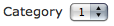
\includegraphics{images/chapter05/config01.png}
    			\caption{Select with id}
    			\label{config01}
    		\end{center}
    	\end{figure}
    	
      Another idea would be to use \texttt{to\_s}. But the default one is not very informative either (fig. \ref{config02}). And
      making developers to redefine \texttt{to\_s} in every model contradicts the entire idea of the plugin being 
      unobtrusive. 
      
      \begin{figure}[hbt!]
    		\begin{center}
    			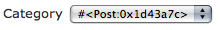
\includegraphics{images/chapter05/config02.png}
    			\caption{Select with to\_s}
    			\label{config02}
    		\end{center}
    	\end{figure}
    	
    	Very similiar situation happens with \texttt{inspect} method which in plain Ruby uses \texttt{to\_s}, but in
    	Rails has been redefined to be a little bit more informative (fig. \ref{config03}). Nevertheless,
      it is not very user friendly in terms of web interface. 
    	
    	\begin{figure}[hbt!]
    		\begin{center}
    			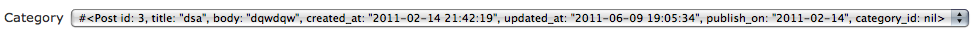
\includegraphics[width=\linewidth]{images/chapter05/config03.png}
    			\caption{Select with inspect}
    			\label{config03}
    		\end{center}
    	\end{figure}
    	
      None of the solutions presented above is correct or even remotely appropriate. Moreover, the application
      is not yet smart enough to tell by itself which fields should be used for display name of given model.
      For human being it is pretty obvious, but machines are not there yet.
      It could require every model to have a field or method name that would be used, but again, that would 
      be the violation of unobtrusiveness rule. Therefore, the user needs some way
      of telling the application, how he wants given model displayed.
      
      In addition, there are much more situations that need some user input - maybe some models of field would be hidden.
      Or some kind of authentication and authorization should be set up for the administer section.
      So, there is a strong need for some kind of configuration. It should be easy enough to still keep the feeling of 
      being "plug and play". User should not be forced to write tedious XMLs or spend more time on it than completely necessary.
      
    \subsection{Domain Specific Language}
      \subsubsection{The idea}
        As said before, forcing developers to define some methods with predefined names is not an option. One of 
        the assumptions of the project was not to interfere with the code of application. So it needs some other 
        way of configuration.
      
        Rails application have special place for things like that. There is a directory \texttt{config/initializers} 
        that is dedicated to hold files that would be loaded during the initialization process of application. 
        They are usually used to set up configuration for gems, plugins and other libraries. This is the place where the user
        would hold configuration for administer.
      
        Another concern was the form that the configuration would take. The first thought was to create the 
        most straightforward way - just provide a set of class methods for \texttt{Administer::Config}
        that would allow people to set appropriate values. One rule could look like that:
      
        \lstinputlisting{code/chapter05/config01.rb}
      
        where \texttt{Category} is the model and \texttt{:name} is the symbol representing method that 
        should be called. 
      
        Looks correct, and probably would be enough for most of use cases. However, soon some developer
        would probably face the fact that none of existing methods or fields are appropriate to display
        as name for the model. Some field may need to be trimmed or the best match would be to combine 
        few fields (eg. first and last name of a person). The immediate solution would be to define the 
        method in model that prepares the name and then pass that to configuration. And as long as that 
        method would be defined and used in the application anyway it is all right. But if it is created
        just for the purpose of using it in configuration it is again kind of situation where some 
        unnecessary code clutters the code of application. Fortunately, Ruby provides an easy way to
        ship functionality that would prevent this. Developers may pass the block, instead of a method name,
        that would get called on the object. Therefore, in case of need for some special actions user could
        define configuration like this:
      
        \lstinputlisting{code/chapter05/config02.rb}
      
        Seems to be much cleaner. Everything that belongs to the plugin is handled apart from the application.
        However, if more options would be handled it starts to gets a little messy:
      
        \lstinputlisting{code/chapter05/config03.rb}
      
        A lot of repeated code and it is easy to imagine what would happen if someone would like to define
        for example 6 options for one model. He would have to write 6 times almost the same thing with just
        changing name of option and method or block for that option. 
      
        So the search for the most suitable solution is still on. But, remembering that it is
        very dynamic environment, some smart outcome can be elaborated. After some deliberations,
        an idea of Domain Specific Language appeared. It could look like this:
      
        \lstinputlisting{code/chapter05/config04.rb}
      \subsubsection{Implementation}
        The great thing is that it is not hard at all to implement such DSL in Ruby. In order to do this
        the only thing needed is understanding the power of blocks and usage of \texttt{eval} function.
        
        The root class is \texttt{Administer::Config}. It provides a class method \texttt{configure} that
        takes one parameter - a block. The only thing that this function does is it creates an object of
        \texttt{Administer::Config} by calling a constructor and passing the block, and after the object
        is created it is assigned to the class variable so that the configuration for application is held
        in one place for entire object space. 
        
        The real work is done in constructor of \texttt{Administer::Config}. Although the code is not
        very long:
        
        \lstinputlisting{code/chapter05/config05.rb}
        
        it shows the power of dynamic programming and to be specific it utilizes the \texttt{instance\_eval}
        method. What this method does is it executes the block in context of the object it has been called on.
        
        So, if there is such piece of code:

        \lstinputlisting{code/chapter05/config06.rb}

        first it creates the object of \texttt{Administer::Config} and then from line 2 the code is executed
        in context of that newly created object. In other words, that code just calls the \texttt{model} in 
        the config object and passes two parameters - class \texttt{Post} and a block.
        
        Then, the situation repeats as the \texttt{model} method creates an instance of class called
        \texttt{Administer::ModelConfig} and the constructor again takes the block 
        and executes it in context of that object. For further details I redirect to the code of application
        in order to dig deeper into its construction.
        
  \section{Routing, Controllers and Html Templates}
    Above has been described internals of the plugin. Now it is time for the more tangible part - the part
    that makes it working on a web and talks to the user via web interface. This part consists of three 
    elements 
    \begin{itemize}
      \item Routing
      \item Controllers
      \item Html Templates
    \end{itemize}
    
    \subsection{Routing}
      The plugin adds following routes to the application (list shows path and HTTP method used for this route)

      \begin{description}
        \item[GET /administer/dashboard] maps to \texttt{index} action of \texttt{DashboardController}. 
          The resulting page shows the dashboard of administer, which at the time is just the list
          of available models with links to models' pages.
        \item[GET /administer/entities] maps to \texttt{index} action of \texttt{EntitiesController}.
          Shows the list of all records of given model. The model name is passed in the parameter
          \texttt{model\_name} so the route would be the following for model called \texttt{Category} -
          \texttt{/administer/entities?model\_name=Category}. All routes that are mapped to \texttt{EntitiesController}
          need this paramaeter.
        \item[GET /administer/entities/new] maps to \texttt{new} action of \texttt{EntitiesController}.
          Used for displaying form for new record of given model. 
        \item[POST /administer/entities] maps to \texttt{create} action of \texttt{EntitiesController}.
          Used for creating new records for given model. Parameters passed should be:
          \begin{itemize}
            \item \texttt{model\_name} as in all entities rotues.
            \item hash named after the model (so for model \texttt{Category} the hash should be called
              \texttt{category}) that contains attributes for the newly created record.
          \end{itemize}
        \item[GET /administer/entities/:id] maps to \texttt{show} aciton of \texttt{EntitiesController}.
          It aims to show details of the record.
        \item[GET /administer/entities/:id/edit] maps to \texttt{edit} action of \texttt{EntitiesController}.
          Used to display form for editing record. The \texttt{:id} variable should contain the id of 
          record that is supposed to be edited. Example route for model \texttt{Category} and id 25:
          \texttt{/administer/entities/25/edit?model\_name=Category}.
        \item[PUT /administer/entities/:id] maps to \texttt{update} action of \texttt{EntitiesController}.
          Parameters are the same as for the route for \texttt{create} action. This route
          aims to update the record with given attributes.
        \item[DELETE /administer/entities/:id] maps to \texttt{destroy} action of \texttt{EntitiesController}.
          It deletes queried record from the database.
      \end{description}
    
      The routes for entities follow guidelines for REST\footnote{Representational State Transfer} architecture.
      This means that it uses rather vocabulary of HTTP for identifying actions instead of elaborating
      some fancy routes to map them to appropriate actions. This is why, the difference between
      \texttt{show} and \texttt{update} or \texttt{destroy} action is just change of HTTP method from \texttt{GET} to
      \texttt{PUT} or \texttt{DELETE} instead of having to routes \texttt{/administer/entities/:id/show} and
      \texttt{/administer/entities/:id/update} or \texttt{/administer/entities/:id/delete}.

      As it can be observed - RESTful architecture encourages to have single URI for managing particular
      resource. \texttt{Edit} and \texttt{new} actions have their own URIs as they are not in fact
      managing the resource - they are only needed for the purpose of displaying appropriate forms
      to users. It is hardly possible, that the user of application would craft appropriate queries
      and parameters himself. But if the user of the application would be another application
      it would not need that additional forms and could handle the resource it needs with 
      single URI.
    
      As a result, the administer part of the application could be easily turned into REST Web Service. 
      Except for normal HTML response, it could be easily extended to send out JSON or XML responses.
    
    \subsection{Controllers}
      As it can be observed in the routing chapter, there are 2 controllers in administer plugin:
      \begin{description}
        \item[DashboardController] handles the actions when the user is not managing 
          any particular model. At the moment it is only \texttt{index} action that displays 
          a list of all possible models.
        \item[EntitiesController] handles user actions when the use is managing
          models. 
      \end{description}
      
      Both of those controllers are subclasses of \texttt{Administer::ApplicationController}.
      
      \subsubsection{ApplicationController}
        The \texttt{Administer::ApplicationController} is the base controller for all of administer controllers.
        Thanks to this fact, it was possible to set up filter that would be active all over administer part of the
        application. This filter would add authentication functionality that can be configured in \texttt{Administer::Config}.

        If a user defines a method for authentication, administer would call it before every request
        for administer part of the application. If any redirect would occur there, it would not proceed
        with actions of administer controllers. Therefore, the developer may define a method that checks 
        whether appropriate user is logged in and if not it would redirect to login page at the same time
        preventing administration section for unauthorized access.
      
      \subsubsection{DashboardController}
       As said above, the functionality of \texttt{DashboardController} at the moment is just delivering
       the index action which, in fact, does not do anything in particular except for rendering the index
       view.
      \subsubsection{EntitiesController}
        \texttt{EntitiesController} is the heart of administer web application. Its responsibility 
        is to handle managing of models. As seen in routes, it provides following actions:
        
        \begin{itemize}
          \item index
          \item show
          \item new
          \item create
          \item edit
          \item update
          \item destroy
        \end{itemize}
        
        The names of the actions are self-explanatory. For all actions there is a filter introduced
        called \texttt{set\_model}, which is used to set up a model before action is started.
        That way it was unnecessary to write the same code for every action.
        The filter takes the \texttt{model\_name} parameter from HTTP query and build a 
        \texttt{Administer::Model} based on that.
        
        For actions that include forms, the controller prepares the list of fields (as described in Fields chapter)
        and puts it in instance variable \texttt{@fields}. It is worth to mention, that all instance variables
        of controller are accessible from view.

    \subsection{Views}
      \subsubsection{Technology}
        The views have been developed using Haml\footnote{http://haml-lang.com/} templating language. It has been chosen 
        over standard ERB because of its cleanliness and conciseness. It requires much less code to produce the same output
        than ERB. For example\footnote{Examples from HAML website} ERBs code:
        
        \lstinputlisting{code/chapter05/views01.erb}
        
        can be transfered to Haml like this:
        
        \lstinputlisting{code/chapter05/views02.haml}
        
        Much less code plus it automatically closes html tags, so it prevents the situation that somewhere in the partial
        a \texttt{div} has not been closed and that affects totally different \texttt{div} somewhere in the layout.
        Debugging of such errors is very tedious and troublesome.
        
      \subsubsection{Structure of views}
        The most outer part of the webpage is held in the layout file that is loaded for every action in every controller.
        So the layout consists of all tags that appear on every web page like \texttt{head} section, opening and closing
        of \texttt{body} tag and so on. The layout has the \texttt{yield} clause. This is the place where templates
        of particular actions are put in.
        
        Every action has its own template named after the name of the action. If some part of the template maybe extracted and used in 
        few places it is put in partial. Partial are named with underscore at the end (eg. \texttt{\_partial.html.haml}). Then
        the partial can be included in the template by using \texttt{render "path\_to\_partial"}.
        
    \subsubsection{Generating of forms}
      The most interesting parts of forms is generating of forms for models. As said before, the controller puts 
      the list of fields for given model in \texttt{@fields} instance variable. The \texttt{edit} and \texttt{new}
      templates first create a form using \texttt{form\_for} method. It just creates the form tag and passes
      the reference to form builder to the block. Then the routine for creating a form starts. 
      
      The list of fields is iterated and for every field \texttt{render field.partial} method is called. The
      \texttt{Administer::Fields::Base} class defines the partial method so that it returns the string - a path
      to the partial. The path is calculated by having the standard path \texttt{administer/fields/} and then
      adding the name of the current class trasnformed to lowercase with underscores to the end of it.
      \texttt{HasMany} becomes \texttt{"administer/fields/has\_many"}. Then, partials for all
      available fields are defined in that path. Every partial defines appropriate html tags
      for given field.
      
    \subsubsection{Styling}
      The administer plugin does not ship any fancy layout. The markup uses appropriate
      ids and classes so that it can be easily customized by the end user. This makes it
      stand out from the collection of available plugins as all of them impose
      some layout. 
      
      Nevertheless, even without setting up any CSS rules the administer plugin looks
      clean, readable and is fully usable. This is because it uses semantic markup, which means
      that it does not use arbitrary tags but those that are the most suitable for the part of 
      the website they describes. Therefore, even if the web browser uses its 
      default rendering rules, the website would be well arranged.
      
  \section{Discussion}
    \subsection{General outcome}
      \label{ch:implementation:general_outcome}
      In general, the project has turned out to be a success. The plugin is functional
      and works as intended. Moreover, the most important aim of making it
      working out of the box (with the little configuration that has been discussed before)
      has been met. 
      
      After creating a Rails application and having \texttt{administer} in the Gemfile
      the application gets \texttt{/administer} path and the user is welcomed with screen
      seen in figure \ref{outcome1}. 
      
      \begin{figure}[hbt!]
    		\begin{center}
    			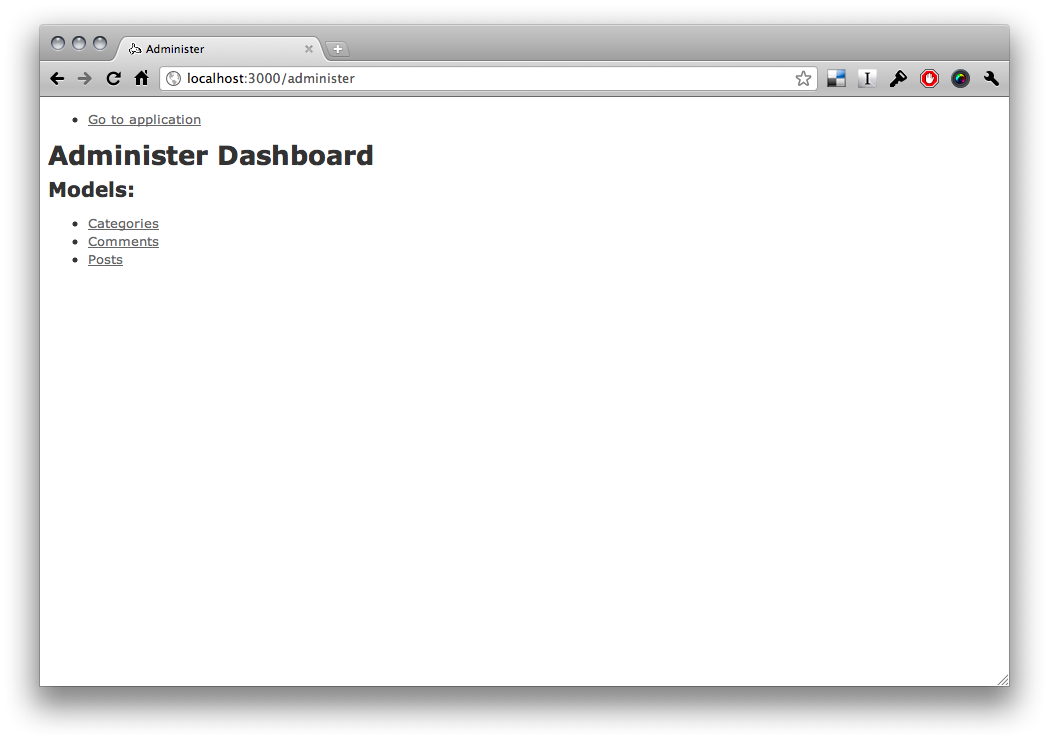
\includegraphics[width = 0.8\linewidth]{images/chapter05/outcome1.png}
    			\caption{Administer Dashboard}
    			\label{outcome1}
    		\end{center}
    	\end{figure}
      
      
      Then while browsing the plugin, the user may browse (fig. \ref{outcome2} p. \pageref{outcome2}) 
      and manage(fig. \ref{outcome3} p. \pageref{outcome3}) his
      models. All actions that have been established at the beginning of the project: 
      browsing, creating, editing and deleting of model records are available and work as intended. 
      
      \begin{figure}[hbt!]
    		\begin{center}
    			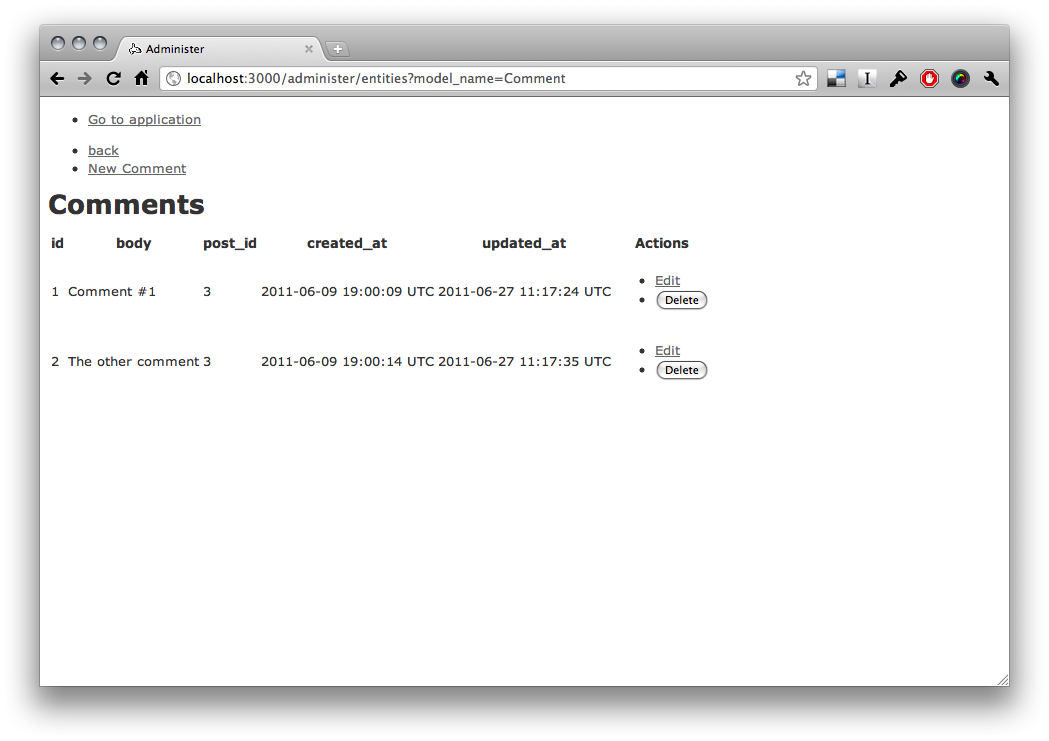
\includegraphics[width = 0.8\linewidth]{images/chapter05/outcome2.png}
    			\caption{Administer list of records}
    			\label{outcome2}
    		\end{center}
    	\end{figure}
    	
    	\begin{figure}[hbt!]
    		\begin{center}
    			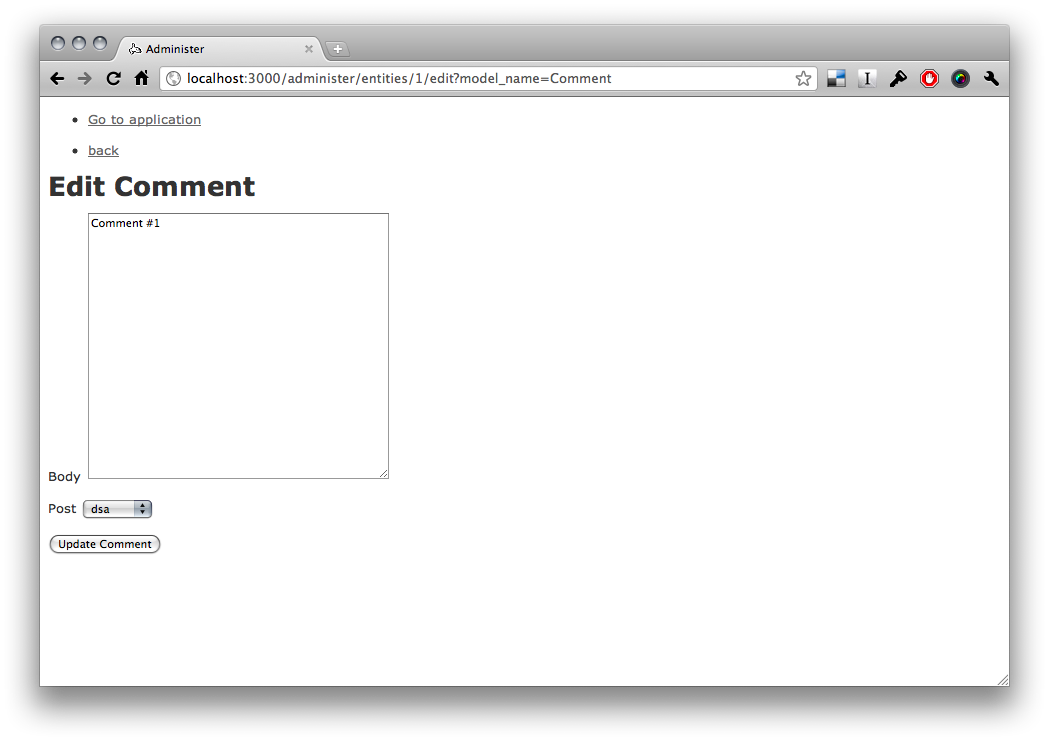
\includegraphics[width = 0.8\linewidth]{images/chapter05/outcome3.png}
    			\caption{Administer: editing record}
    			\label{outcome3}
    		\end{center}
    	\end{figure}
      
    \subsection{Unsolved problems}
      \label{ch:implementation:unsolved_problems}
      There are still some unsolved problems in the application. Fortunately, none of them
      cause the plugin to be non-functional and they are rather wishes for the improvement.
      
      First of all, it still in some places is bound to ActiveRecord. 
      Though, it was not an aim of the project to make it totally independent of ActiveRecord 
      and the plugin has been developed for ActiveRecord based test application, it would be nice
      to decouple it and introduce totally modular binding to ORM. 
      
      Moreover, the configuration is very simple at the moment. It is really hard to
      guess all the options people would want. But, the implementation of configuration
      is pretty open and it would be easy to introduce new options to the DSL once
      people start using it and posting requests.
      
      The list of records could have been improved. As the rendering of forms
      have been thought through, and a lot effort has been put into making it
      work, the view that lists records is using very simple implementation. Probably
      some thought should be put there in order to make it more error prone and more 
      easily customizable.
      
      In the end, handling of \texttt{:through} associations would be a nice feature.
      Through associations are defined when one model is associated to another one 
      via some intermediate model. Such associations are not yet handled here as
      some additional research would need to be conducted in order to find out
      how people would like to use it.
      
      